%
% prozessrauschen_geaendert.tex -- Kombination der Prozessrauschen-Bilder
%
% (c) 2021 Prof Dr Andreas Müller, OST Ostschweizer Fachhochschule
%
\documentclass[tikz]{standalone}
\usepackage{amsmath}
\usepackage{times}
\usepackage{txfonts}
\usepackage{pgfplots}
\usepackage{csvsimple}
\usetikzlibrary{arrows,intersections,math}
\begin{document}
\newboolean{showgrid}
\setboolean{showgrid}{false}
\def\skala{1}
\begin{tikzpicture}[>=latex,thick,scale=\skala]

\node at (0,0) {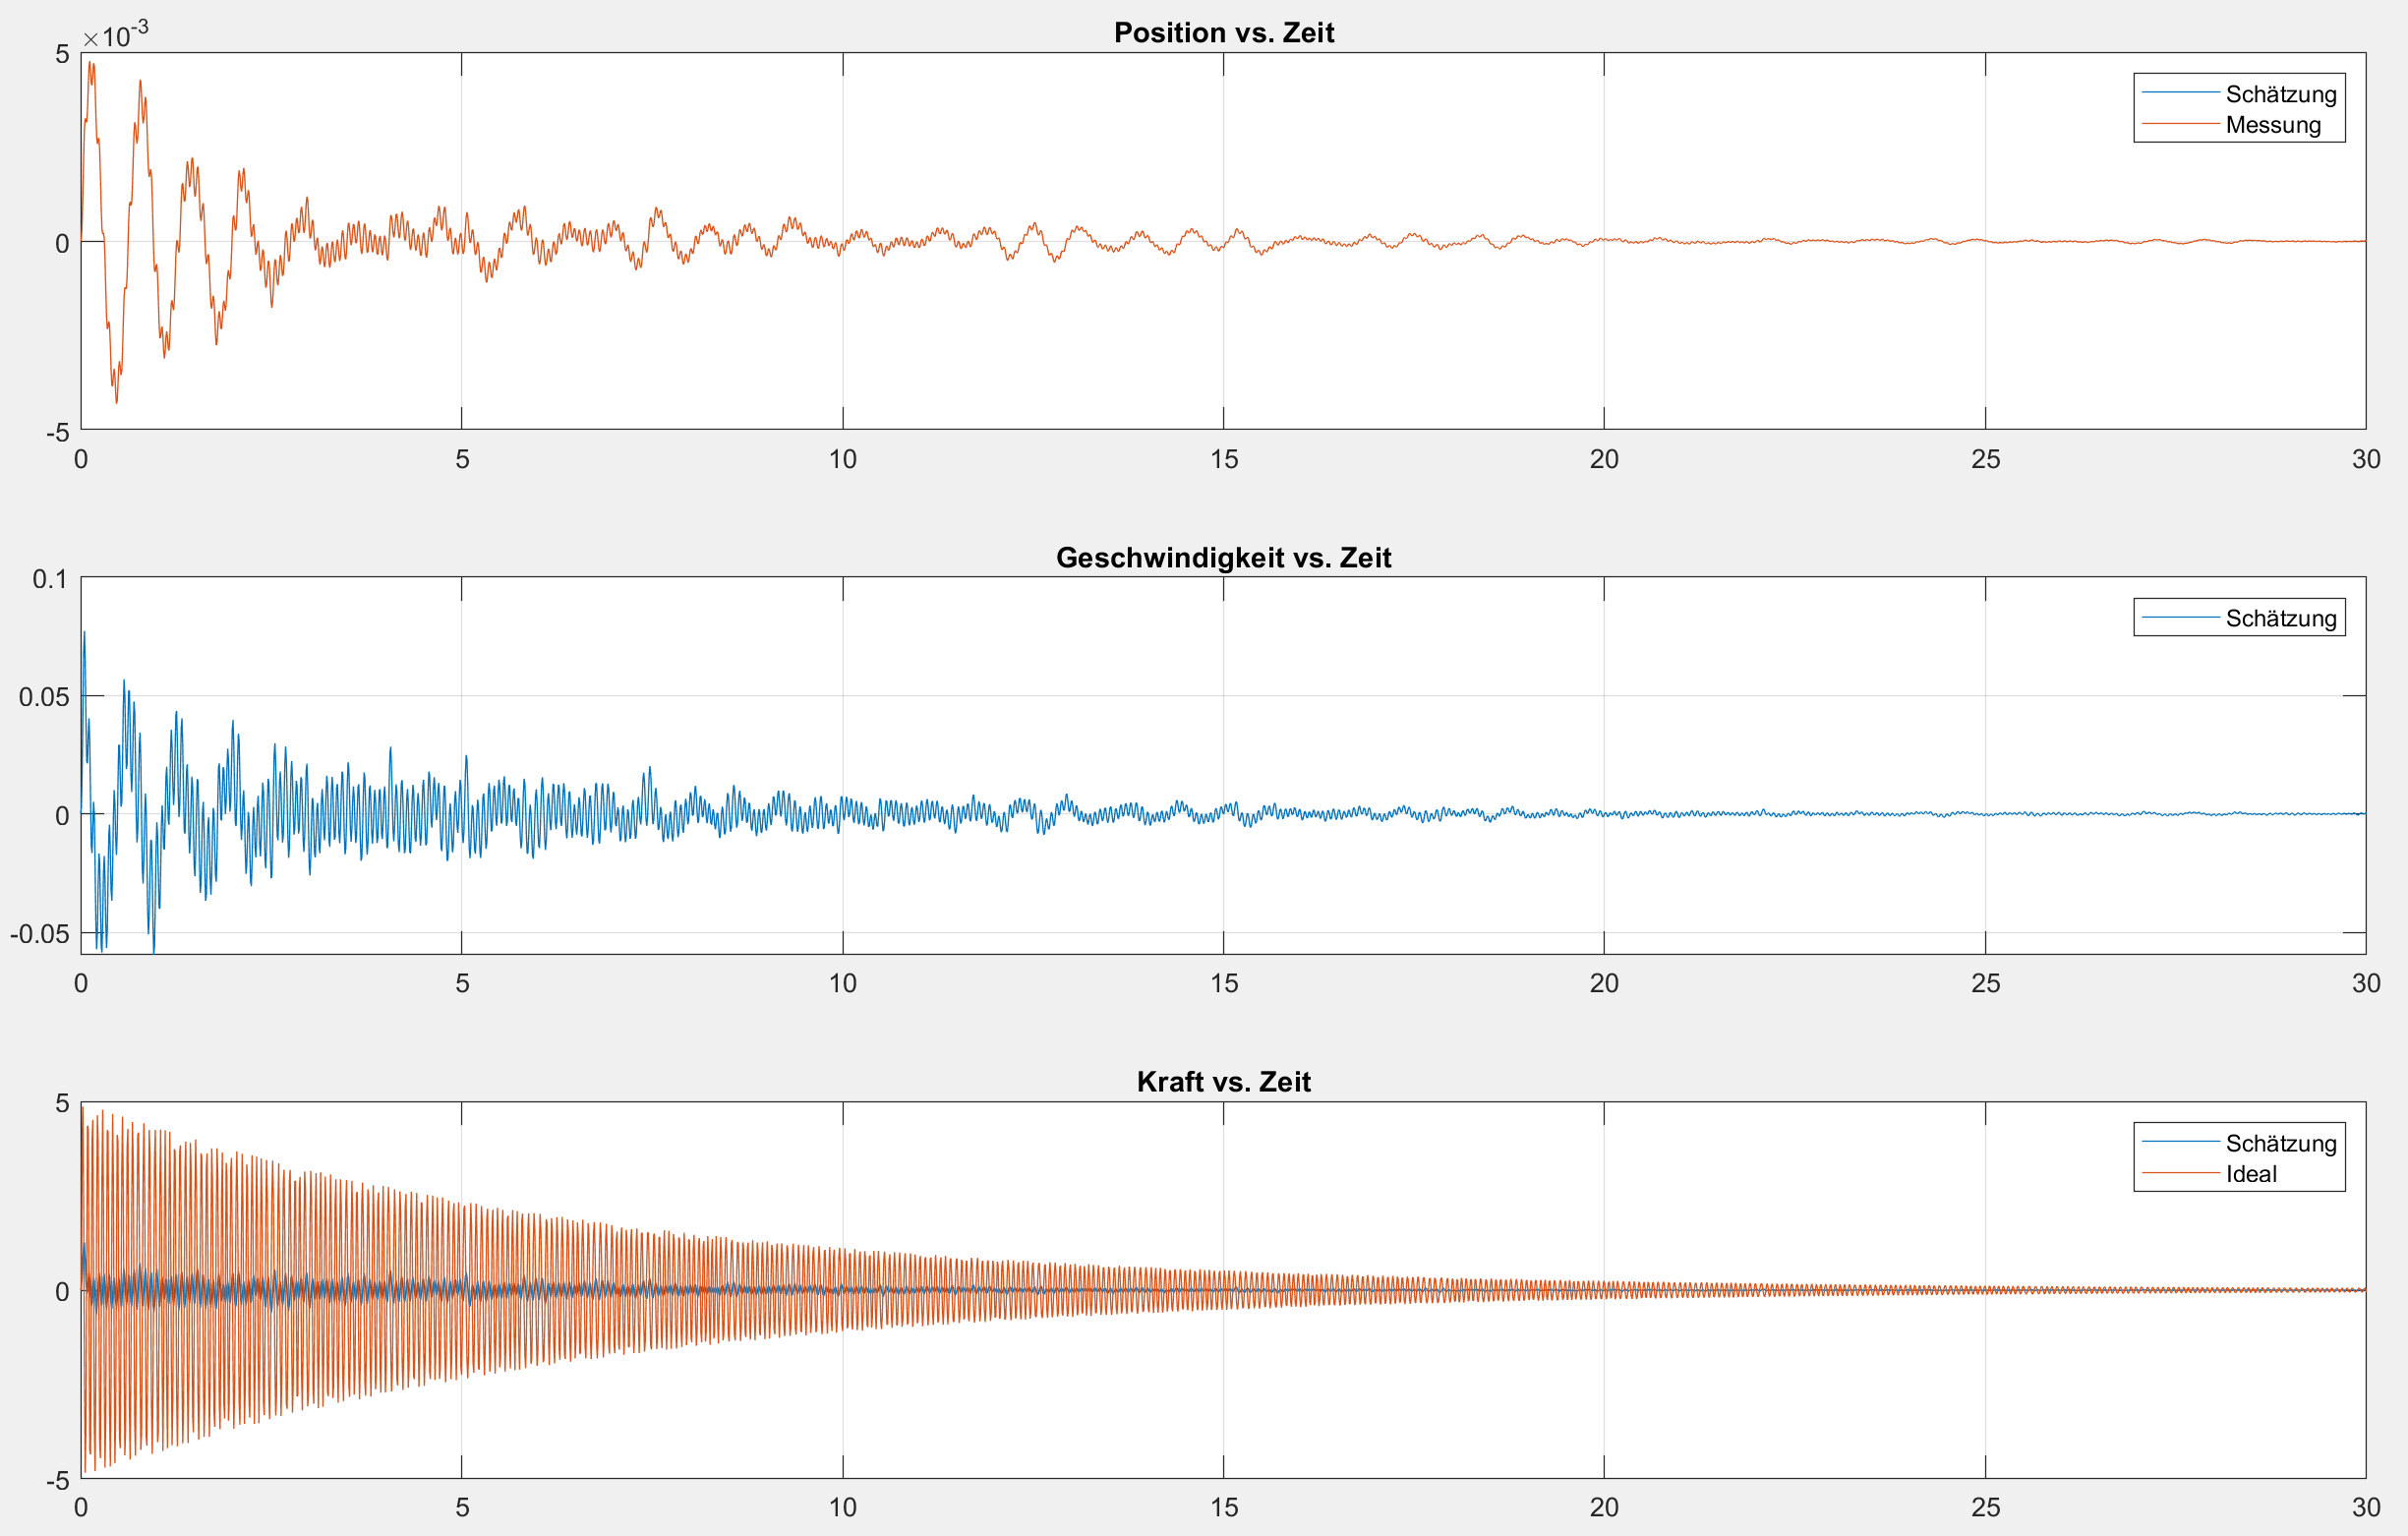
\includegraphics[width=14cm]{../Prozessrauschen_geaendert.PNG}};

\def\yten{-2.1}
\def\yfifteen{0.12}

\def\links{13.27}
\def\rechts{14.2}

\pgfmathparse{(\yfifteen-(\yten))/5}
\xdef\m{\pgfmathresult}
\xdef\b{\yten}

\pgfmathparse{\m*(\links-10)+(\b)}
\xdef\Links{\pgfmathresult}

\pgfmathparse{\m*(\rechts-10)+(\b)}
\xdef\Rechts{\pgfmathresult}

\begin{scope}[yshift=-9cm]
\node at (0,0) {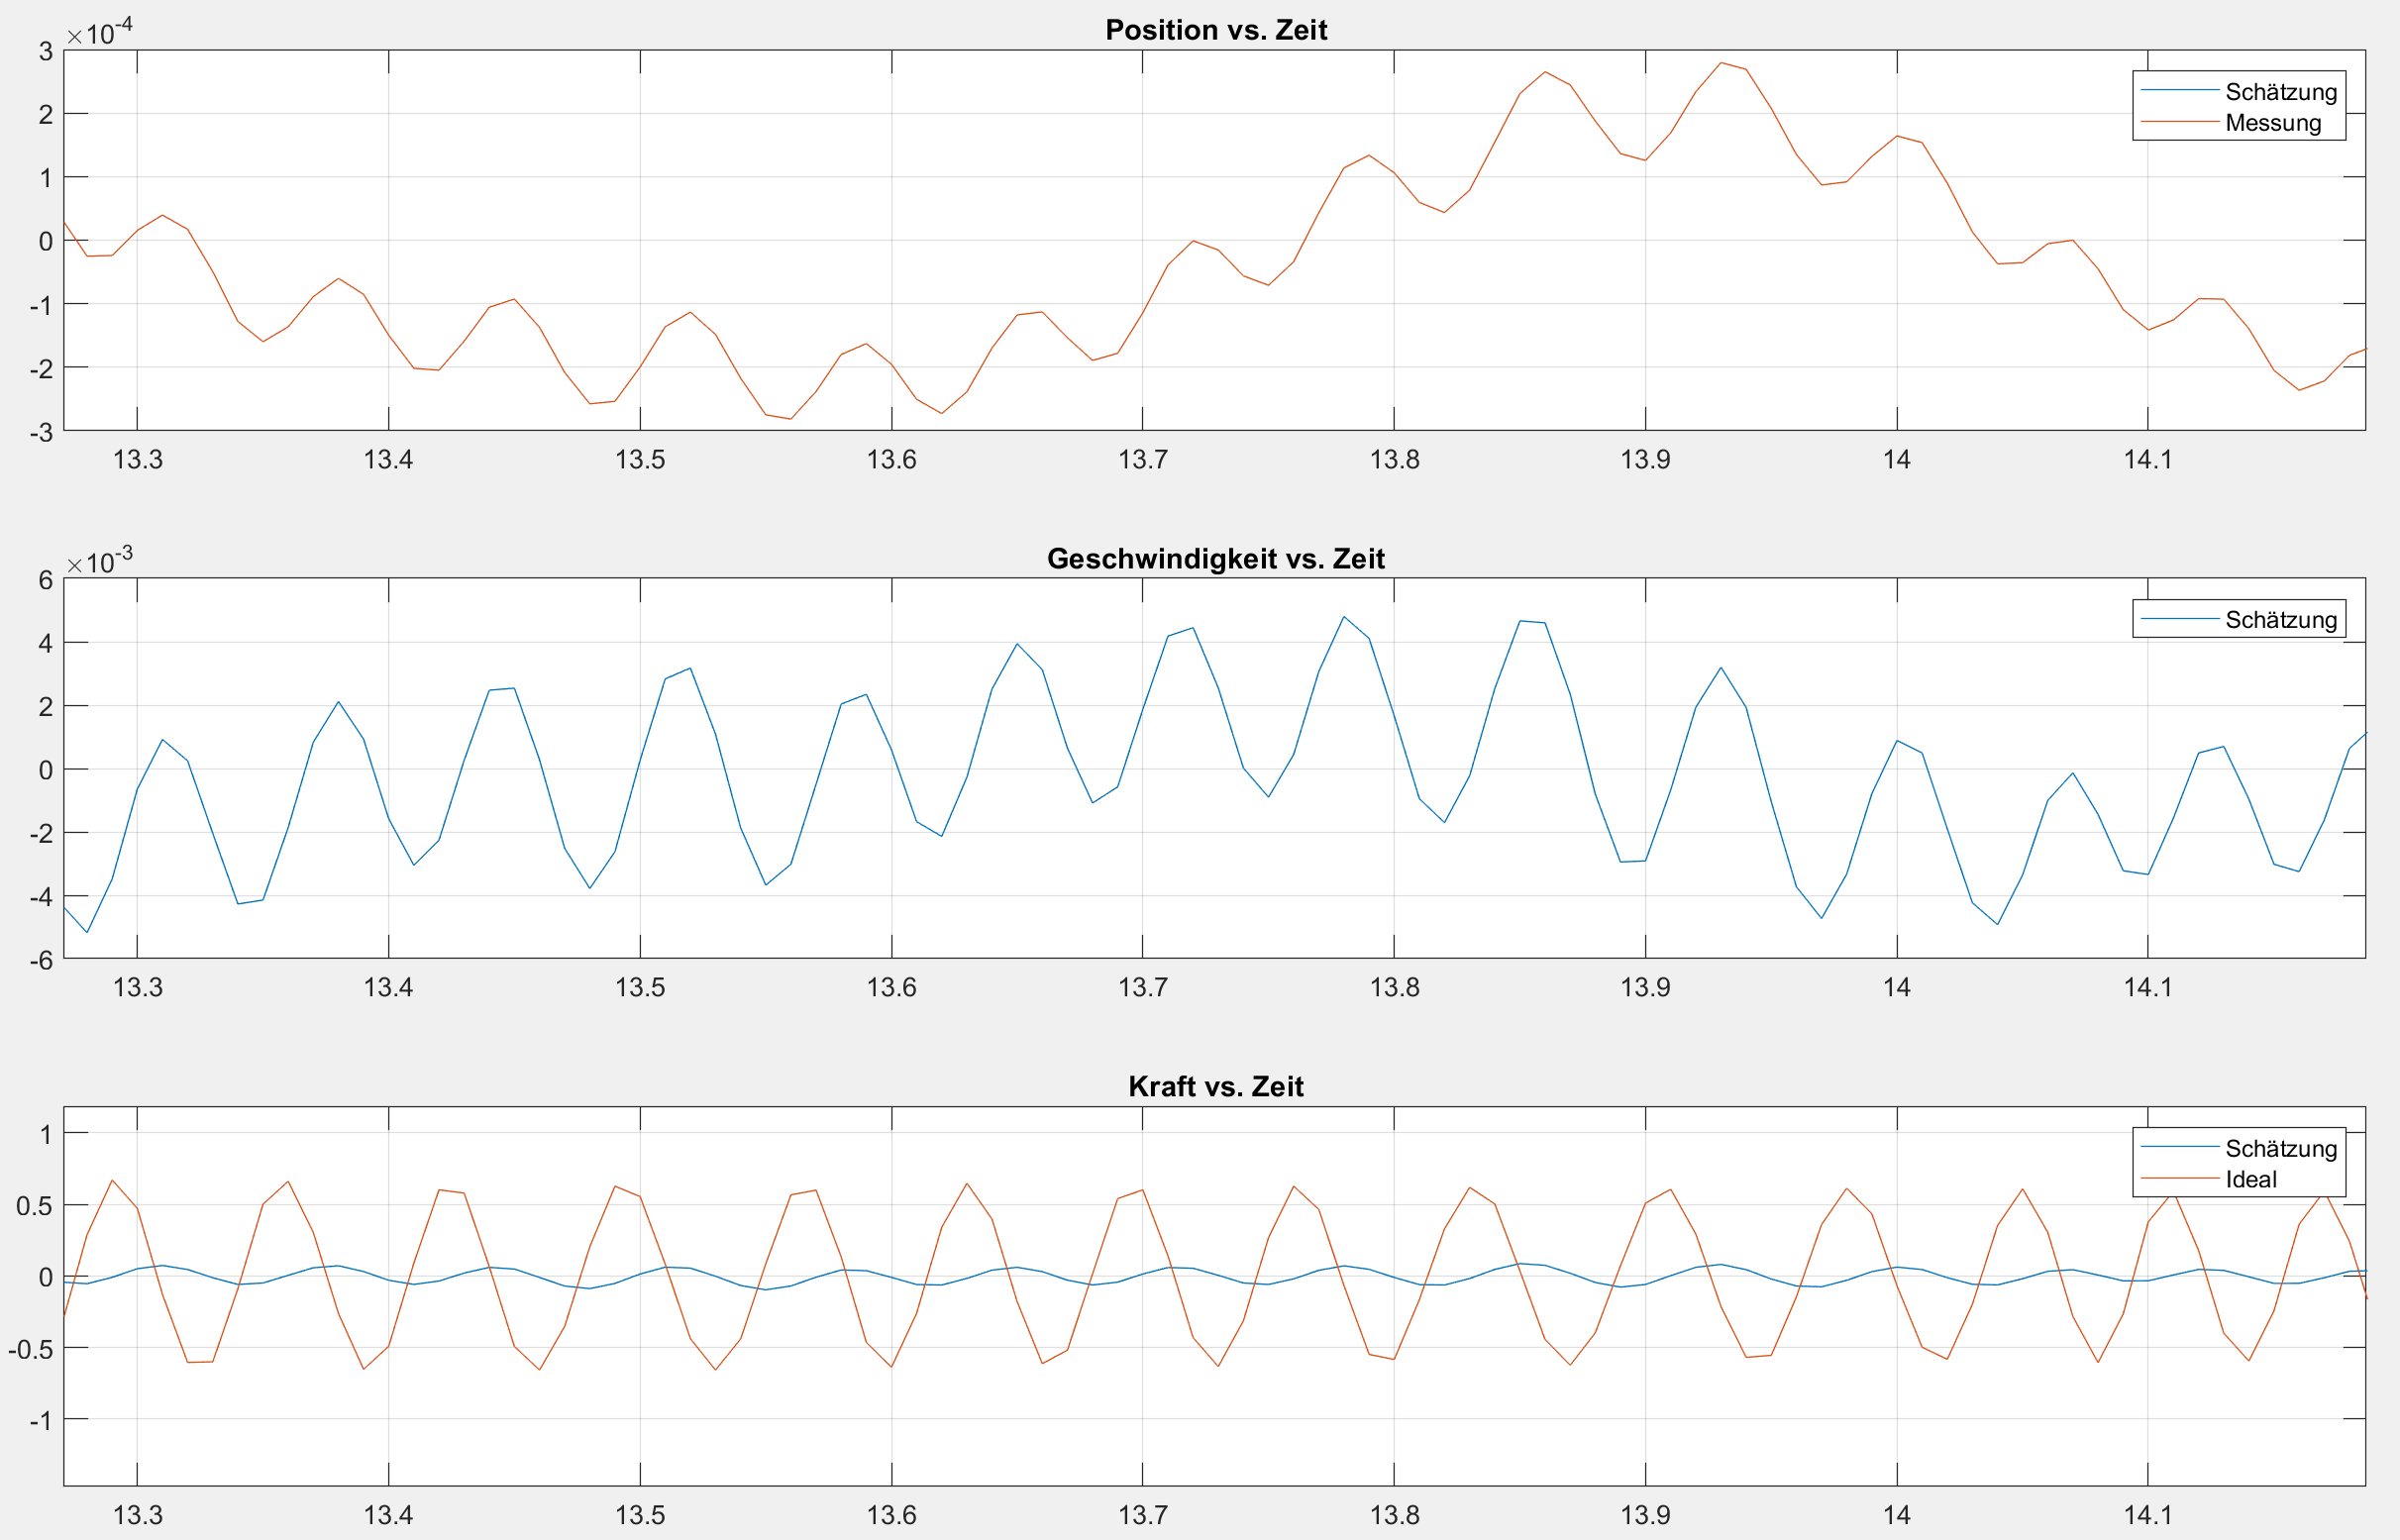
\includegraphics[width=14cm]{../Prozessrauschen_geaendert_zoom.PNG}};
\end{scope}

% Gitter
\def\breite{7}
\def\hoehe{2}
\ifthenelse{\boolean{showgrid}}{
\draw[step=0.1,line width=0.1pt] (-\breite,-\hoehe) grid (\breite, \hoehe);
\draw[step=0.5,line width=0.4pt] (-\breite,-\hoehe) grid (\breite, \hoehe);
\draw                            (-\breite,-\hoehe) grid (\breite, \hoehe);
\fill (0,0) circle[radius=0.05];
}{}

\def\unten{-4.15}

\draw[line width=0.7pt] (\Links,\unten) rectangle (\Rechts,4.18);
\draw[line width=0.7pt] (\Links,\unten) -- (\Links,{\unten-0.05})
	-- (-6.62,-4.6) -- (-6.62,-4.9);
\draw[line width=0.7pt] (\Rechts,\unten) -- (\Rechts,{\unten-0.05})
	-- (6.80,-4.6) -- (6.80,-4.9);

\end{tikzpicture}
\end{document}

